\chapter{利息度量}
\begin{introduction}
	\item 累积函数
	\item 贴现
	\item 利息力
\end{introduction}
		\section{累积函数}
	\begin{definition}{累积函数}
\noindent 	时间零点的1元在时间t的累值,记为 $a(t)$
		\end{definition}
\begin{property}
  \noindent  (1) $a(0)=1$\\
(2) $a(t)$ 通常是时间的增函数\\
(3) 当利息连续产生时, $a(t)$ 是时间的连续函数
\end{property}
	\section{贴现}
	\begin{definition}{贴现}
\noindent	$v=\frac{1}{1+i}$ \\ $d=iv$\\ $i=\frac{1}{v}-1$
	\end{definition}
\begin{note}
i:利率,v:贴现因子,d:贴现函数
\end{note}
\begin{definition}{利息力}
\noindent		设可积函数连续可导,则称
\[
\delta_{t}=\frac{a^{\prime}(t)}{a(t)}=[\ln a(t)]^{\prime}
\]
为时刻 t 的利息力
		\end{definition}
		\\ 衡量利息增长速率与利息本身大小的比值
		很有意思的是,我们把t当做横坐标的时候,相当于t是定下来的,以这个为标准来用利息力来计算累积函数
		$$\int_{0}^{t} \delta_{s} d s=\int_{0}^{t} \frac{a^{\prime}(s)}{a(s)} d s=\int_{0}^{t}[\ln a(s)]^{\prime} d s=\ln a(t)$$
		\begin{property}
		$$\ln \left(a\left(t_{2}\right)\right)-\ln \left(a\left(t_{1}\right)\right)=\int_{t_{1}}^{t_{2}} \delta_{t} d t \text { or } a\left(t_{2}\right)=a\left(t_{1}\right) e^{\int_{t_{1}}^{t_{2}}\left(\delta_{t}\right) d t}$$
\\We can also write, assuming that $a(0)=1$
\[
\ln (a(t))=\int_{0}^{t} \delta_{\tau} d \tau \text { or } a(t)=e^{\int_{0}^{t} \delta_{\tau} d \tau}
\]
\end{property}
\begin{property}
	累积函数:\\
\[
a(t)=\exp \left(\int_{0}^{t} \delta_{s} d s\right)
\]\\
 贴现函数:\\
\[
a^{-1}(t)=\exp \left(-\int_{0}^{t} \delta_{s} d s\right)
\]
	\end{property}
Timeline:a essentail point of view for problem-solving \\
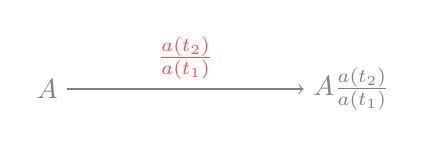
\begin{tikzpicture}
\draw [color=black!50,->](0,0) node[left]{$A$}-- node [color=red!70,pos=0.5,above,sloped]{$\frac{a(t_2)}{a(t_1)}$}(3,0) node[right]{$A\frac{a(t_2)}{a(t_1)}$};
 \end{tikzpicture}
\begin{example}
compound interest:$a(t)=(1+i)^t$\\
$$A \cdot \frac{a\left(t_{2}\right)}{a\left(t_{1}\right)}=A(1+i)^{t_{2}-t_{1}}$$
\end{example}
\begin{example}
simple interest:$a(t)=1+it$\\
$$A \cdot \frac{a\left(t_{2}\right)}{a\left(t_{1}\right)}=A \cdot \frac{1+i t_{2}}{1+i t_{1}}$$
\end{example}
\
$$(1+\frac{i^{(n)}}{n})^{n}=(1+\frac{i^{(m)}}{m})^{m}$$
\begin{exercise}
	在第1月末支付314元的现值与第18月末支付271元的现值之和,等于在第T月末支付1004元的现值.年实际利率为$5\%$. 求$T$
\end{exercise}
\begin{solution}
$$1004 v^{T / 12}=314 v^{1 / 12}+271 v^{18 / 12} \Rightarrow T=141.6$$
\end{solution}